%===================================== KAPITTEL 2 =================================

\chapter{Teori}
% Først, introduser og definer begrepet ''aggregatorientert datamodell'' - Kanskje jeg bør forklare ytterligere hva det betyr?
Ifølge \cite{sadalage2013} kan nøkkelverdilagre (eng. key-value store), kolonnefamilielagre (eng. column family stores) og dokumentlagre (eng. ''document stores'') ordnes under én og samme ''art'' av NoSQL-databaser: Aggregatorienterte databasesystem (eng. ''aggregate oriented databases''). Denne introduksjonen til de tre nevnte NoSQL - datamodellene forholder seg til denne klassifiseringen. Utover disse tre typene av NoSQL - modeller finnes også den graforienterte modellen, som benyttes av systemer som InfiniteGraph, OrientDB og FlockDB. Denne datamodellen vil ikke bli beskrevet i noen videre detalj. Det bør nevnes at med begrepet ''datamodell'' menes den programmatiske metoden data organiseres av et DBMS, i vitenskaplig notasjon er ''metamodell'' mer presist.

% Dette kapitlet presenterer litteraturoversikten og resultater fra prosjektarbeidet
Dette kapitlet gir leseren en innføring i tre NoSQL - datamodeller, hvordan de skiller seg ut fra den relasjonelle datamodellen og hvordan deres forskjeller fra relasjonelle databaser har innvirkning på hvordan levende oppgradering av dem og migrasjon av eksisterende data i produksjonsmiljøet kan utføres i en smidig utviklingsprosess.

Vi begynner med å beskrive den relasjonelle datamodellen, og hvorfor den ikke holder mål i et distribuert produksjonsmiljø der større datavolum behandles. Dernest blir den aggregatorienterte datamodellen presentert, en kategori underordnet NoSQL-paraplyen som denoterer fellesnevneren mellom nøkkelverdilagre, dokumentlagre og kolonnefamilielagre. Samtlige tre former for aggregatorientering beskrives i avsnitt 2.2.1 til 2.2.3.

% Om den relasjonelle datamodellen
% Før første subseksjon: ; 2.1.3: Nøkkel-verdi-lagre; 2.1.4: Dokumentlagre; 2.1.5: KFL; 2.1.2 Ett eget overordnet kapittel om aggregatorientering; 2.1.1 mySQL?
% 2.1 - Om relasjonelle modeller, motivasjonen bak NoSQL
\section{Den relasjonelle datamodellen}

% Den relasjonelle datamodellen, i.e. MariaDB og Postgres (Bøyningen av sybstantivet 'tuppel' samsvarer med Bratsbergengens skrivemåte i hans artikkel om relasjonsdatabaser hos SNL)
For å forstå framveksten av NoSQL - databaser er . I den relasjonelle datamodellen organiseres forskjellige former for applikasjonsdata inn i relasjoner, og data tilhørende samme relasjon inndeles i atomiske, disjunkte enheter kalt \emph{tupler}. En tuppel er en flat, endimensjonal liste av dataverdier. Hver av disse verdiene korresponderer til nøyaktig ett attributt av relasjonen tuppelen er lagret i.

% Strukturelle begrensninger i relasjonsdatabaser
Det foreligger visse begrensninger på denne datastrukturen. Til eksempel kan ikke en enkelt tuppel nøstes inn i en annen, og hvert attributt i tuppelen har én atomisk korresponderende verdi, aldri en liste av verdier. Nå skal det sies at nyere versjoner av MariaDB støtter JSON-objekter som datatype \citep{mariadb}. JSON-objekter er serialiserte (dsv objekter konverterte til strenger), fleksible dataenheter som kan inneholde nøstede datastrukturer.

Imidlertid har ikke databasesystemet noen forståelse for de enkelte dataelementer som objektet innkapsler, det ser bare en helhetlig, ugjennomsiktlig dataenhet, nemlig verdien av ett attributt i relasjonen. Ettersom tupler er den minste, udelelige dataenheten i den relasjonelle modellen er det korrekt å fastslå at spørringer opererer med og returnerer (et helt antall) tupler for hver enkelt spørring \citep{sadalage2013}. Riktignok går det an å utvelge distinkte attributter i spørringen, også kjent som kommandoen \texttt{PROJECT} i relasjonell algebra, likefullt er den tellbare dataenheten i resultantrelasjonen tupler, også referert til som rader i kontekst av databaseapplikasjoner.

% Spørringsfleksibilitet (JOIN + avanserte operasjoner) - Fra databasepensum
Følgelig gir slike strengt strukturerte datamodeller stor fleksibilitet for spørringene som utføres av databasesystemet. Det kan for eksempel samle sammen alle verdier for ett spesifikt numerisk attributt i én bestemt relasjon, summere disse  attributtverdiene sammen og returnere resultatet som et separat attributt i resultanttuppelen. På samme vis kan relasjonsdatabasesystemet kalkulere gjennomsnittet for alle eller enkelte av tuplene i en relasjon, telle opp antallet tupler i den, finne den høyeste numeriske verdien eller finne den laveste.

Ved hjelp av JOIN-operasjoner finner man eksisterende tupler fra forskjellige relasjoner, relatert til hverandre via fremmednøkler, og resultanten av JOINen kan systemet også kalle disse aggregeringsoperasjonene på. NoSQL - databaser har ikke den samme fleksibiliteten til selv å utføre slike spørreoperasjoner: Hver spørring henter kun én dataenhet ad gangen, noe som holder især for nøkkelverdilagre. Hver spørring er logisk sett bare et oppslag på en nøkkel i en hashtabell. Eventuell aggregering der sum, gjennomsnitt eller ekstremalverdier regnes må gjøres i selve applikasjonen, etter at oppslag på \textbf{samtlige} nøkler er gjort i databasen.

% Figur 1
\begin{figure}[ht]
    \centering
    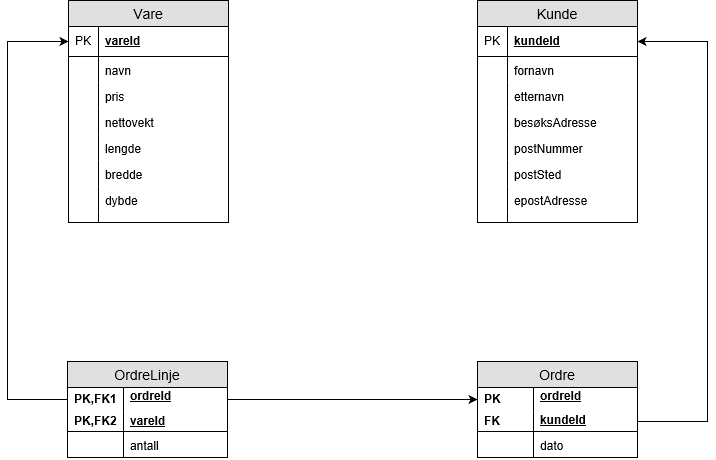
\includegraphics{fig/NettbutikkOrdreModell.png}
    \caption{Diagram over tabeller i en relasjonsdatabase som registrerer ordrer fra kunder i en netthandelapplikasjon.}
    \label{fig1}
\end{figure}
 
\subsection{Impedansproblemet (Impedance mismatch problem)}

I en typisk netthandelapplikasjon er applikasjonens datamodell denotert i form av dataobjekter midlertidig lagret i primærminnet, mer presist sagt, i adresseområdet til èn, eller flere, av nettleserens kjørende prosesser i kundens datamaskin. Variablene i datafeltene i disse objektene kan være saå mangt: strenger, tall, referenser til andre objekter, lister bestående av ovennevnte typer. Disse dataobjektene endres i sanntid av kunden som aksesserer nettbutikken gjennom standardiserte interaksjonselementer som tekstfelt, knapper, slidere, sjekkbokser og radiobokser, gruppert sammen i dynamiske sideelementer kjent som skjema (eng. ''form''). Et praktisk eksempel på et skjema i en netthandel er handlevognen, som viser kunden hvilke vareartikler han (foreløpig) vil kjøpe, hvor mange av hver vare som ''ligger'' i handlevogna, og hvor mye varene koster sammenlagt.

Når det kommer til å skrive dataene fra web-skjemaet til disk i en relasjonsdatabase ser ting annerledes ut. Her persisteres data om varer (navn, identifikasjonsnummer, størrelsesdimensjoner, nettovekt, og enhetspris \footnote{Gitt at hver enkelt vare-tuppel representerer en diskret enhet, til eksempel én bøtte maling eller én sekk med poteter}) til en egen relasjon. En annen relasjon holder data om kunder, en tredje holder på informasjon om bestillinger, og for normaliseringens skyld eksisterer en egen jointabell kalt Ordrelinje som kopler sammen Ordre og Vare, som illustrert i tabell-diagrammet i \ref{fig1}. Denne uoverensstemmelsen mellom strukteren av applikasjonsdata i programminne og strukturen på de samme dataene i en relasjonsdatabase refereres til i industrien som ''the impedance mismatch'' \citep{sadalage2013}.

Følgelig må applikasjonsutviklere konvertere data fra spørringsresultater til den dataobjektstrukturen applikasjonen påkrever, noe som per idag ofte løses ved å innføre et seperat abstrahert lag i applikasjonens logiske arkitektur: En tredjepartsmodul kalt ''object-relational mapper'' (ORM). For språket Java kan man bruke Hibernate\footnote{\url{http://hibernate.org/orm/}}, JavaScript har SequelizeJS\footnote{\url{http://docs.sequelizejs.com/}}, og PHP-utviklere kan bruke Doctrine\footnote{\url{http://www.doctrine-project.org/}}, som også er en del av webapplikasjonsrammeverket Symfony\footnote{\url{http://symfony.com/}}. Med slike tredjepartsbibliotek følger selvfølgelig et nytt mønster som utviklere blir nødt til å forholde seg skal de ta det i bruk. Ettersom det relasjonelle datalaget abstraheres bort er det tilforlatelig å ''glemme'' at applikasjonsdata faktisk persisteres i en relasjonell database. En tilsynelatende enkel henteoperasjon på objektform kan fort translatere til to kostbare JOIN-operasjoner i databasen som kjøres hver gang spørringen utføres.

% Distribuering av data utover flere instanser == katastrofe
En annen innvending mot den relasjonelle datamodellen involverer hvordan den støtter skalering av arbeidslast med hensyn på økende antall brukere, økende antall datakilder, og økende spørringsfrekvens databasesystemet utsettes for. Datamodellen ble etablert på 70-tallet, i en æra lenge før distribuert databeregning tok av i bedriftsmarkedet. Relasjonsdatabaser er designet med tanke på monolittiske systemarkitekturer, programvarearkitekturer hvis system kjører på én enkel datamaskin, fordelt på et sett med prosesser innad i den. For et begrenset antall datakilder/brukere er slike systemer i noen grad vertikalt skalerbare, det vil si at økt last på systemet kan løses ved å oppgradere maskinvaren. Denne metoden er innlysende nok kostbar i det lange løp ettersom maskinvare som skiftes ut ikke er brukelig for systemet lengre. Da er det billigere å skalere horisontalt, det vil si å kjøre programvaresystemet i en klynge av datamaskiner sammenkoplet over et IP - nettverk. Hver av disse datamaskinene er billige, altså består de av maskinvarekomponenter som yter dårligere enn den jevne stordatamaskin som prosesserer banktransaksjoner.  Som demonstrert i følgende eksempel statuert av \cite{george2011} skal vi se at å operere i klynget system ikke er så lett når data modelleres relasjonelt.

% Jamfør HBase - penusm i TDT4150
\subsection{Hush}

Hush er en (fiktiv) url-forkortelsestjeneste som i begynnelsen har omtrent et par tusen brukere, og vedlikeholdes og bygges med gratis tredjepartsmoduler, blant annet driftes en LAMP-tjener (Linux, Apache, MariaDB, PHP) som leverer en prototype av denne tjenesten i form av en webapplikasjon. Hush sin relasjonelle databasemodell normaliserer sine data ved å definere fire tabeller, \texttt{user}, \texttt{url}, \texttt{shorturl}, og \texttt{click} \citep{george2011}. De tre sistnevnte tabellene er assosiert med \texttt{user} gjennom en fremmednøkkel som refererer til nøkkelattributtet til den tabellen. I tillegg er brukertabellen og kort-URL-tabellen indeksert etter sine respektive nøkkelattributter for å gjøre oppslag på korte URLer og brukere raskere. Ved å sluse endringer inn i systemet som transaksjoner sikrer man at de relaterte tabellene (den for URLer, korte URLer og klikk) endres sekvensielt og fullstendig uavhengig av hvor samtidig de uavhengige skriveoperajsonene forekommer slik at et strengt konsistensnivå opprettholdes tuplene imellom.

Transaksjoner er en velprøvd og høyt akseptert logisk modell for databehandling. Relasjonelle databaser tillater oppdatering av eller lesing av tupler i opptil flere relasjoner innen et sett med atomiske operasjoner. Det er den enkelte mengden av hendelser som heter for en transaksjon. En transaksjon avgrenser mengden av hendelser og skriver enten samtlige eller ingen endringer til disk.

Transaksjonenes egenskaper beskrives med akronymet ACID: De er atomiske, dvs at samtlige hendelser i transaksjonen blir enten gjennomført fullstendig eller ei; konsistente (eng. ''Consistent''), dvs at to transaksjoner som kjører parallellt alltid medfører det samme sluttresultatet; isolerte, det vil si holdbare i den grad transaksjonen persisteres til disk (eng. ''Durable''). Transaksjonsmodellen fremmer en spesifikk handling, \texttt{COMMIT}, som signaliserer at endringene spesifisert i den enkelte transaksjon er blitt gjort permanente.

Denne monolittiske databasearkitekturen fungerer med det gitte antall brukere. Idet tjenesten blir verdenskjent, og antallet brukere øker eksponensielt med fire tierpotenser, blir arbeidslasten for databasetjeneren etter hvert for stor å handtere alene. Den naturlige løsningen på å tekkes vekstraten i databasens arbeidslast er å innføre flere databasetjenere installert på separate datamaskiner. Når skriveoperajsoner og leseoperasjoner i et databasesystem distribueres utover en klynge tjenere, er det viktig å organisere dem slik at arbeidslasten av skrivinger og lesinger jevnfordeles metodisk slik at databasesystemets distribuerte natur ikke er synlig for applikasjonen som utfører spørringen. En vanlig organiseringsmetode er master-slave-replikering, der én master-tjener mottar alle skriveoperasjoner for å serialisere dem \citep{george2011}.

I historien om Hush er dette veien dets utviklere tar: Slavetjenerne får motta lesespørringer, én enkel mastertjener fordeler skriveoperasjoner blant slavene. Hush er en applikasjon der leseoperasjoner utnummerer skriveoperasjoner i antall, det hender jo oftere at noen klikker på en frokortet lenke snarere enn at noen poster en lenkeforkortelse på tjenesten. For en stakket fungerer denne lastfordelingen utover klyngen, men etterhvert er tilveksten av brukere såpass stor at leseoperasjonene samlet sett blir trege. Etter hvert blir også masterdatabasetjeneren som handterer samtlige skriveoperasjoner blir en flaskehals i systemet \citep{george2011}.

For å øke ytelsen til leseoperasjonen installerer utviklerne av Hush et distribuert hurtiglager med det minnebaserte nøkkelverdilageret Memcached\footnote{\url{https://www.memcached.org/}}. Imidlertid svekkes oppdateringskonsistensnivået til systemet ettersom dataverdier i hurtiglageret må skiftes ut etter hvert som transaksjoner behandles av mastertjeneren. For å holde tritt med den økende skrivelasten kunne man oppgradere mastertjenerens maskinvare, altså å skalere oppover, en lite bærekraftig løsning i lengden ettersom det finnes et øvre fysisk tak på antallet mikrotransistorer som kan få plass innen én kvadratmillimeter mikrochip. Det er også en svært kostbar, fordi slavetjenernes maskinvare må nødvendigvis også oppgraderes i lengden for å holde tritt med de stadig innkommende skriveforespørslene fra mastertjeneren. På toppen av disse bekymringene går også utførelse av JOIN - operasjonene for tregt for at systemene skal kunne holde tritt med den økende frekvensen av spørringer fra applikasjonstjenerne, så man velger da å denormalisere tabellene. Det er nå kommet tydelig fram at den relasjonelle datamodellen nå er til mer bry enn den er til hjelp for Hush-utviklerne.

Av denne historien kan man oppsummere at relasjonelle databasesytemer ikke er laget for å kjøre i et distribuert miljø. Ei heller lar de seg skaleres horisontalt, altså at løsningen på økende arbeidslast er å legge til en datamaskin med billige maskinvarekomponenter i et distribuert nettverk av andre liknende datamaskiner og jevnfordele spørringene utover dem. En relasjonsdatabasetjener kan istedet skaleres vertikalt, det vil si at prosessorenheter med høyere klokkefrekvenser og minnekort og harddisker med større datakapasitet installeres i tjenermaskinen og erstatter de gamle. Ikke bare er dette en utålelig dyr løsning, men den forårsaker også i vedlikeholdsperioder, dog bytte av maskin i dag tar stadig kortere tid hos dagens skytjenester, der appliakjsonen ikke kan betjene noen brukerforespørsler. For å takle lagring og behandling av stadig større datavolum, må vi se nærmere på en annen, nyere og mer fleksibel måte å strukturere lagret data på. 



% Om NoSQL
% 2.2
\section{Den aggregatorienterte datamodellen}

Så har vi den aggregatorienterte modellen, en metamodell som tillater den enkelte systemarkitekt å selv definere kompleksiteten til strukturen til sine egne dataenheter, slik at persisterte data er tilpasset applikasjonens struktur på sine dataobjekter i stedet for å tvinge vedkommende til å konformere med en forhåndsbestemt minste enhet, slik tilfellet er i den relasjonelle modellen. Denne fleksibiliteten i struktureringen av data er et sentralt fellestrekk nøkkelverdilagre som Dynamo og Redis deler med kolonnefamilie-lagre som Cassandra og HBase og dokumentdatabaser som MongoDB og CouchDB. Derfor definerer \cite{sadalage2013} en felles kategori for disse tre NoSQL-typene: ''Aggregatorienterte databasesystem''.

Begrepet ''aggregat'' (må ikke forveksles med det matematiske verbet som betegner en operasjon på en gruppe av tupler) er lånt fra domenedrevet design og er i kontekst av databasemodellering definert som en samling sammenknyttede objekter som en datamodellør ønsker å behandle som en enhet for datamanipulasjon og konsistenshandtering. Når komplekse aggregater aksesseres, gjøres det med et oppslag på én enkelt nøkkel, så får man både dataobjektet med den tilhørende nøkkelen samt eventuelle assosierte dataobjekter. Å utføre en tilsvarende lesing av to assosierte relasjoner i for eksempel MySQL krever først oppslag i en tabell på dens nøkkelverdi, deretter enda et oppslag på en fremmednøkkel i den assosierte tabellen, altså må en JOIN-operasjon utføres.

En aggregatmodell avgrenser den objektsrukturen til applikasjonens data som skal alltid skal omskrives i ett sett, hvilket betyr at når data i et nøstet objekt endres, blir hele aggregatobjektet i seg selv omskrevet. Aggregatet utgjør dermed en naturlig enhet for replikering i et distribuert databasesystem da hele den aggregerte objektstrukturen programvarens forretningslogikk jobber innenfor replikeres i sin helhet. En tuppel i en normalisert relasjon inneholder nødvendigvis ikke hele omfanget av dataobjektstrukturen forretningslogikken arbeider på, iallfall ikke uten en eller to JOIN-operasjon.

Aggregatobjektet er også en naturlig enhet for partisjonering: En stor mengde av individuelle aggregater er fra programvaresystemet sitt sitt standpunkt aksessert fullstendig uavhengig av hverandre, derfor kan de lemfeldig fordeles og kopieres utover et sett med uavhengig opererende databasenoder uten at objektenes plassering får konsekvenser for applikasjonens aksessmønster - skal en klient ha tak i ett spesifikt objekt kan den i prinsippet kontaktet én spesifikk databasenode i nettverket som er kjent for å holde på dette ønskede objektet. Å partisjonere tabeller i et relasjoner distribuert databasesystem kan, avhengig av de rådende assoiasjoner og fremmednøkkelbegrensninger, påvirke ytelsen til forskjellige spørringer etter forskjellige tupler som tilhører samme tabell, på grunn av algoritmen den distribuerte JOIN-operasjonen er implemntert med så vel som plasseringen av tupler med matchende assosiasjonsvariable (lik verdi for fremmednøkkel og primærnøkkel).

Lesing av aggregerte dataobjekter medfører at man med ett enkelt oppslag på én enkel nøkkel får både i pose og sekk. Aggregatmodellen er også en enklere datamodell å forholde seg til for de som programmerer selve applikasjonen som behandler dataene, av den enkle grunn at de slipper å skrive kode for å konvertere en lemfeldig liste av flate tupler. De enkelte aggregater, det vil si applikasjonsprogrammererens definisjon for databehandlingsenhet utgjør en naturlig enhet for replikering i en klynge av enkeltstående databasenoder. I et distribuert databasesystem gjelder det å minimalisere antall noder som kontaktes for hver spørring. Når konsepter settes sammen eksplisitt i datamodellen slik som vi ser i de fleksible dokumentstrukturene til Mongo, vet databasen hvilke dataenheter som skal aksesseres samtidig, og som derfor naturlig nok bør plasseres på én og samme node.

\cite{sadalage2013} kaller relasjonelle databaser og grafdatabaser for \textbf{aggregat-uvitende}. Deres datamodeller betrakter ikke aggregater eller sammensatte datastrukturer i deres dataoperasjoner. Aggregat-uvitenhet er ikke nødvendigvis et dårlig designvalg, ettersom det ikke alltid er opplagt for den enkelte webapplikasjonsutvikler hvilke enhetsbegrensinger i datamodellen som er logiske, iallfall ikke før datamodellen er definert for første gang og revidert to til tre ganger i løpet av utviklingsprosessen. Den lagrede dataen kan ha mange forskjellige brukskontekster, avhengig av applikasjonens funksjonelle krav som ofte blir forandret underveis i applikasjonens livssyklus.

En enkelt aggregatstruktur kan ikke medføre optimale spørringsytelse for alle mulige brukskontekster. Her gjelder det for utvikleren å prioritere den mest typiske leseoperasjonen tjenesten utsettes for. Hvis applikasjonen ikke har en slik primær aksess – struktur på dataobjektene kan man like godt modellere dem på et aggregat-uvitende vis. I en aggregat-uvitende modell har brukskonteksten ingen innvirkning på spørringen, fordi operasjonsenheten er én enkelt tuppel i MariaDB uansett hvordan konseptene er satt sammen.

Aggregatorienterte databasesystemer innehar ikke ACID - egenskapene som vi finner hos transaksjoner i relasjonelle databasesystemer. Imidlertid støtter de naturlig atomiske manipulasjoner på ett eneste aggregat av gangen. Ved nøkkeloppslag får man hele dataobjektet den tilkoplete applikasjonen leser og manipulerer, Samtidighetskontroll ved operasjoner på flere aggregater må følgelig handteres i kildekoden til applikasjonen, spørring for spørring, der et unntak må kastes hvis én av spørringene mislykkes. Å emulere transaksjoner i enkeltaggregater inngår som en viktig faktor i hvordan aggregatene defineres i datamodellen \citep{sadalage2013}.

% 2.2.1
\subsection{Design av aggregatmodeller}

% DDI: Denormalisering, duplisering og intelligentte fremmednøkler

% Legg inn eksempel av aggregatmodell konvertert fra figur 1
Slik kan en generisk aggregatmodell, uttrykt i UML, ekvivalent til datamodellen fra \ref{fig1} se ut.

% Figur 2
\begin{figure}[ht]
    \centering
    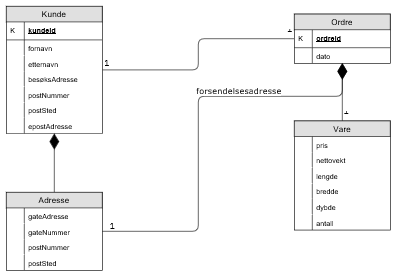
\includegraphics{fig/NettbutikkAggregatModell.png}
    \caption{Aggregatdiagram med to forskjellige entiter for den samme tjenesten fra \ref{fig1}.}
    \label{fig2}
\end{figure}

Denne figuren  presenterer to forskjellige aggregater, \texttt{Kunde} og \texttt{Ordre}. Forbindelsen mellom disse to denoterer 
Ved modellering av aggregater må man avveie mellom hvor stort hvert enkelt aggregatobjekt i en applikasjon kan bli og hvor mange forskjellige aggregatentiter applikasjonen kan ha. Med to nivaåer av nøstede lister av objekter innen ett aggregat kan besvarelse av ett enkelt oppslag på én spesifikk nøkkel 

% Skriv om tre ulike aggregat - orienterte datamodeller - Segway til påfølgende delkapitler
Fowler og Sadalage omtaler tre unike datamodeller som opererer med aggregater. Nøkkelverdimodellen behandler det enkelte aggregat som en ugjennomsiktig helhet \citep{sadalage2013}. Altså går det ikke an å hente deler av aggregatet ved et nøkkeloppslag. Dokumentmodellen eksponerer aggregatet til databasen, og tillater dermed delvise spørringer. I og med at dokumentmodellen også er skjemaløs går det ikke an å optimalisere spørringer på hele eller deler av aggregatet. Kolonnefamilier inndeler aggregatet i grupper, noe som tillater databasen å operere på hver av disse gruppene som en egen dataenhet, lik som attributter i tuplene i den relasjonelle modellen. Selv om kolonnefamilier til dels ofrer den komplette skjemaløsheten som vi ser i nøkkelverdimodellen, har databasen nå mulighet til å nytte eksponeringen av attributter/kolonner til å optimalisere aksesseringer og oppdatere separate kolonner.

% 2.2.2
\subsection{Nøkkel-verdi-modellen}

Nøkkelverdilagre er den type NoSQL-DBMS med den enkleste datamodell. Spørringer inndeles hovedsaklig i tre kategorier: GET, PUT og DELETE. 


% Teorien som legger til grunn for Project Voldemort
\section{Amazon Dynamo}

% Introduksjon/Abstract
\cite{decandia2007} presenterer arkitekturen til Dynamo, et høytilgjengelig, distribuert nøkkel-verdi-lager som ved nettverkspartisjoner ofrer replikakonsistens til fordel for å være mottakelig for lese - og skriveforespørsler fra diverse mikrotjenester som lever i Amazons applikasjoner. I kjernen av problemet denne distribuerte databasearkitekturen forsøker å løse ligger et sterkt krav til at enhver kunde av Amazons netthandel alltid skal kunne legge artikler i handlekurven. Handlekurven i nettbutikken, så vel som hver eneste artikkel i nettbutikken skal til enhver tid kunne interageres med. Ethvert avbrudd i denne tjenesten kan og vil medføre monetære tap enten direkte i form av utsatte handler og indirekte i form av øøkende mistro hos forbrukerne. Amazon.com er samlet sett en gigantisk, distribuert netthandelapplikasjon bestående av mange tusen nettverkskomponenter og uavhengige tjenere spredt utover mange datasentre. I denne infrastrukturen er feil som oppstår i enkeltkomponenter normen, ikke unntaket.

% Hva er motivasjonene bak utviklingen av systemet / What is the motivation for the research/development?
Amazon.com er en av verdens største netthandelplattformer. På det meste handler 10 millioner brukere fra verden over på nettbutikken samtidig. Hvis ett av lagene i tjenestearkitekturen påkrever vedlikeholdsarbeid går det ikke an å ta ned hele nettbutikken fullstendig for så mye som en time uten å tape en uutholdelig mengde penger.

% Hvilket problem løser Dynamo? / What is the domain (area) of the problem being solved?
% Hva er artikkelens hovedbidrag? / Which techniques are developed (presented) in the paper?
% What are the implications applications of Dynamo? / konsekvenser?

% Styrker og svakheter
Dynamos ring av noder som lagrer data er et likemannsnettverk. Et likemannsnettverk er en distribuert programvarearkitektur der alle noder utfører de samme arbeidsoppgavene.

% Teknikker:
%   Consistent Hashing
%   Quorum-spørringer
%   Konflikt - resolusjon: Hvorfor bruke vektorklokker når man like så godt kan bruke Lamport-klokker/tidsstempler?

% Om Project Voldemort
\section{Project Voldemort}

Project Voldemort er et distribuert nøkkelverdilager inspirert av Amazons nøkkelverdilager Dynamo, hvis arkitektur presenteres av \cite{decandia2007}. Dette systemet replikerer og partisjonerer dets data automatisk. Forfatterne og vedlikeholderne \footnote{Kildekoden til Project Voldemort er lisensiert under Apache 2.0 - lisensen, og er tilgjengelig på følgende GitHub-repositorium: \url{http://github.com/voldemort/voldemort/tree/master}} av kildekoden refererer til Voldemort som en stor distribuert, persistent, feiltolerant hash-tabell \citep{kreps2009}. Hver enkelt node i det kjørende databasesystemet holder en delmengde av den totale datamengden som handteres. Flere komponenter i dette systemet er valgfrie – databasemotor, plasseringsstrategi for data-tupler, og serialiseringsmetoden er valgfrie for den enkelte programmerer, alle tre. Blant annet kan man bruke lagringskomponenter som InnoDB, RocksDB (som benytter LSM-trær), Berkeley DB, eventuelt kan man lagre tupler i primærminnet. I tillegg er også nivået på konsistens av skriveoperasjoner justerbart. Prosessperspektivet til arkitekturen er master-fri, det vil si at i det distribuerte datalageret holdes det ikke valg av spørringskoordinator blant nodene, som derfor opererer som et likemannsnettverk. Hvis feil oppstår ved spørringseksekvering blir de behandlet transparent.

\subsection{Støttede operasjoner}
Nøkkelverdilagre tilbyr tradisjonelt sett et svært enkelt spørregrensesnitt til applikasjoner som bygger sine datamodeller med dem. Og Voldemort er overhodet ikke annerledes i den forstand. Dets applikasjonsprogrammeringsgrensesnitt definerer hovedsakelig tre funksjonelle endepunkter: \texttt{get} (leseoperasjoner), \texttt{put} (skriveoperasjoner, både til opprettelse og oppdatering av tupler), og \texttt{delete} (sletteoperasjoner). I tillegg til disse tre operasjonene som er karakteriske for de fleste nøkkelverdilagre definerer Voldemorts klient – API endepunktene \texttt{getAll}, som er en leseoperasjon på multiple nøkler, og versjonerte utgaver av \texttt{get} og \texttt{put} som til forskjell fra de ordinære funksjonene med samme navn tar inn et versjonsobjekt som input til funksjonen i tillegg til en nøkkel og en verdi, slik at tjeneren slipper å gjøre et oppslag for å finne den nyeste versjonen til det angitte objektet først. Hvis versjonen av objektet hvis nøkkel er spesifisert i funksjonskallet ikke er den nyeste vil klientprogrammet kaste et unntak, kalt \texttt{ObsoleteVersionException}, og brukeren får ingenting returnert. Som tidligere nevnt i den generelle diskusjonen om nøkkelverdilagre anser en databasenode hos Voldemort både nøkkel og det assosierte dataobjekt som en lemfeldig sekvens of bytes.

Som et interressant apropos eksponerer \emph{StoreClient} - grensesnittet til Voldemorts kildekode en tredje type \texttt{get} og \texttt{put}: En variasjon som tar inn en transformsfunksjon som kjøres av databasenodene som mottar disse spørringene før (put) eller etter (get) de oppdater eller henter sitt eget datareplika. Disse funksjonene er nyttige for den som vil implementer en Voldemort-databaseklient i Java som kan migrere data levende hvis det implisitte skjemaet til den ovenstående webapplikasjonen blir endret.

\subsection{Voldemorts egenskaper sammenliknet med RDBMS}
I forhold til relasjonelle databasehåndteringssystemer er Voldemort vesentlig bedre egnet til å innføre replikering av data, da ytelsen til både leseoperasjoner og skriveoperasjoner lar seg skalere horisontalt. Det vil si at hvis en ny node legges til det distribuerte miljøet, også benevnt i litteraturen som ''databaseinstansen'' \citep{sadalage2013}, så vil det ha ingen eller neglisjerbar påvirkning på ytelsen. 

Et relasjonelt DBMS har den fordel over Voldemort at dets innebygde samtidighetshåndtering, som utføres ved hjelp av transaksjonsmønsteret, er strengere og derfor mer pålitelig enn Voldemort, som fokuserer heller på å holde orden på endringshistorikken til hver enkelt tuppel som lagres på den enkelte node i det distribuerte lageret. Ved hjelp av versjonering kan kopier, eller replikaer, av tupler hvis dataverdier er divergerende rettes opp gjennom en flettingsprosess.

Moderne webapplikasjonssystemer består gjerne av forskjellige, adskilte tjenester eller applikasjonsgrensesnitt, hver av disse kan i sin tur distribuere egne data over opptil flere datasentre rundt om i verden. Slike webapplikasjoner kan ikke ta seg tid til å vente på JOIN - operasjoner mellom to entiteter eller tabeller som potensielt ligger på hver sin MySQL - tjener på hver sin datamaskin i hvert sitt datasenter på to vidt forskjellige lokasjoner på kloden. Én framgangsmåte på å skalere en relasjonell datamodell til å møte behovene til flere tusen forespørsler samtidig er å introdusere et hurtiglager - nivå i systemarkitekturen ved hjelp av et distribuert, minnebasert cachesystem som MemCache eller Redis for å avlaste databasen for leseoperasjoner som vil utgjøre en flaskehals for den samlede ytelsen til den distribuerte applikasjonen. Dessverre vil ikke denne løsningen skalere for skriveoperasjoner og JOIN - operasjoner så lenge logisk konsistens for skrivinger er et krav. Voldemorts løsning, hvis tekniske detaljer vil bli diskutert i neste delkapittel, er å lempe på disse konsistenskravene.

Relasjonelle databasesystemer realiserer de assosiasjoner som er spesifisert mellom entitetene i datamodellen til applikasjonens arkitektur, og oppfyller samtidig fire egenskaper for skriveoperasjoner som gjøres i systemet gjennom konvensjonen transaksjoner: Atomisitet, en garanti på at hver enkelt transaksjon enten utføres fullt og helt eller avbrytes; Konsistens: for hver enkelt utførte transaksjon etterlates databasen i en konsistent tilstand; Isolasjon: Hver enkelt transaksjon kjøres uavhengig av hvilke andre transaksjoner som kjøres samtidig; Holdbarhet: Data som er persistert gjennom transaksjoner i systemet vil ikke endres eller forsvinne med mindre påfølgende transaksjoner gjør så. Hver enkelt PUT i Voldemort er atomisk så lenge det opererer på et og samme aggregat i datamodellen, det vil si den komplekse objektverdien som aksesseres med nøkkelen.

Transaksjoner gjør skriveoperasjoner i relasjonelle databaser lineariserbare, som er det strengeste konsistensnivået skriveoperasjoner kan ligge på i databasesystem, ved å tvinge skriveoperasjonen til å vente hvis den prøver å endre rader eller tabeller som allerede er reservert for en tidligere påbegynt transaksjon. Voldemort, på sin side legger seg på et mildere konsistensnivå, kalt svak konsistens (eng. ''eventual consistency'').

\subsection{Konsistenskontroll og versjonering}
I likhet med Amazon Dynamo er også Voldemort sin replikakonsistenskontroll inspirert av quorumsystemer. Quorumreplikering og Dynamos liknende replikeringsstrategi av det beskrives i \ref{dynark}.

Likesom i Dynamo tillater Voldemort samtidige skriveoperasjoner på samme nøkkel på forskjellige noder. Begrunnelsen for dette valget er at Dynamo er alltid mottakelig for skriveoperasjoner \citep{decandia2007}, slik at for eksempel en handlekurv alltid kan oppdateres i sanntid. Følgelig kan to eller flere replikaer for samme nøkkel være lagret på forskjellige uten å være synkroniserte, det vil si at ingen av de to replikaene har den fulle og hele oppdateringshistorikken til nøkkelen. I stedet for å preservere replikakonsistens i systemet for alle nøkler til enhver tid, går både Dynamo og Voldemort for å forsone divergerende replikaer for en og samme nøkkel når den blir \texttt{get}-et av applikasjonen, en prosess kalt ''read repair'' av \cite{decandia2007}.

Hvert dataobjekt som skrives tillegges en vektorklokkeverdi som del av dets metadata. Ved en leseforespørsel på samme nøkkel kan koordinatoren for denne leseforespørselen motta replikaer med divergerende vektorklokkeverdier, også kalt \emph{versjoner} \citep{kreps2009}. Hvis systemet er i stand til å forsone og flette oppdateringshistorikken til nøkkelen basert på vektorklokkeverdiene til replikaene, så vil spørringskoordinatoren returnere én gjeldende dataverdi tilbake til klienten som sendte leseforespørselen. Samtidig vil koordinatoren sende skrivespørringer til hver av replikanodene til nøkkelen slik at de kan oppdatere sitt replikaobjekt med den flettede verdien. Hvis en slik forsoning ikke er vil vil koordinatoren returnere alle de konflikterende versjonene av aggregatet til appliaksjonsklienten slik at den utføre den samme fletting med applikasjonens semantikk, som databasen ikke er kjent med hensyn til den logiske separasjonen av ansvarsområder. Applikasjonen vil deretter persistere den definitive, sammenflettede versjonen av aggregatet tilbake til datalageret.

\subsection{Serialisering av dataobjekter}
Innen datateknologi er serialisering prosessen der objekter eller datastrukturer i datamaskinminne som holder på applikasjonsdata konverteres til et format som lar seg lagres på disk, eventuelt forsendes over et nettverk. I en datamaskins interne minne kan relaterte dataobjekter, det vil si objekter som aksesseres av en og samme programvareprosess, ligge på vidt forskjellige minneadresser. Hvis disse dataobjektene skal forsendes over et I/O - grensesnitt er det viktig å samle dem sammen og ordne dem på et vis som kan leses av en datamaskin, derav begrepet serialisering. Serialisering går som regel ut på å flatpakke en nøstet datastruktur, for eksempel et tre, et objekt, eller en matrise, til en enkelt-dimensjonal sekvens av binære sifre. Den konverterte strengen av bits blir da enten persistert til disk eller sendt til en helt annen datamaskin over et IP - nettverk. Ved mottak eller lesing fra disk blir bit-strengen konvertert tilbake til den opprinnelige datastrukturen. Serialisering kan også brukes i eksterne prosedyrekall (RPC).

Serialisering av minnebaserte datastrukturer er en ganske vanlig oppgave i distribuerte systemer og applikasjonsprotokoller, og derfor kan dette gjøres i mange programmeringsspråk. I Java blir klasser som implementerer grensesnittet java.io.Serializable automatisk serialisert. I Python brukes modulen pickle fra standardbiblioteket til samme formål. I PHP nyttes funksjonen \texttt{serialize()} til serialisering og \texttt{unserialize()} til parsing. I JavaScript er JSON - objektet, med dets to metoder \texttt{parse()} og \texttt{stringify()} innebygd i språket. JSON - protokollen er nemlig basert på et subsett av JavaScript. Følgelig kan en hvilken som helst datastruktur formet i JSON - syntaksen oversettes til JavaScript - syntaks.

Hos Voldemort serialiseres dataobjekter før de lagres. Ved å serialisere data kan man garantere at datalageret er helt og holdent uvitende om hva det er sekvensene av 1-ere og 0-ere som blir lagret står for. Applikasjonsutviklere som benytter Voldemort som sin database kan bruke en av mange forskjellige teknikker, eventuelt implementere sin egen. Serialisering sies å være -pluggbart- i Voldemort, slik at man står fritt til å bruke serialiseringsrammeverk som Apache Avro, Googles ProtoBuf, Apache Thrift og Javas serialiseringsgrensesnitt som tidligere nevnt \citep{kreps2009}. Ved hjelp av serialisering kan komplekse datastrukturer som lister og navngitte tupler benyttes som både nøkler og verdi for de enkelte rader.

\subsection{Lastbalansering av dataobjekter}

I et klynget databasesystem er det viktig å fordele datareplikaer slik at databasenodene i klyngen hvver holder på omtrent like stort datavolum til enhver tid. For skalerbarheens skyld kan ikke én eneste node holde på samtlige dataobjekter som lages i databasen, ellers vil datautilgjengeligheten være inversproporsjonal med antallet tjenere i klyngen.

% Konsistent hashing i implementasjon av Voldemort
Konsistent hashing - teknikken brukes også i Voldemorts lastbalanseringsalgoritme, og i likhet med Amazon Dynamo er konsistent hashing en sentral algoritme som brukes for å oppnå jevn fordeling av nøkler, også kalt ''tokens'' av \cite{decandia2007}, så vel som implementering av den quorumaktige replikeringsalgoritmen og rebalansering av datalasten idet databasernoder kommer inn i og går ut av ringen. I en ''tradisjonell'' hashalgoritme hashes data eller nøkler inn i binært rom bestående av et fast, forhåndsinnstilt antall \emph{partisjoner}, eller bøtter. Hver av disse partisjonene handterer et forhåndsinnstilt del av det binære verdiområdet (et tall fra 0 til en stor toerpotens minus 1) til hashfunksjonen.

% Ved svikt i node
Når en node svikter permanent, vil dets datalast bli omdistribuert til de gjenværende nodene i ringen hvis partisjoner grenser mot de partisjonene av ringen den feilede noden hadde ansvar for, altså omaddresseres aggregater tidligere lagret av en nå feilet og permanent utilgjengelig node. Noder med høyere lagrinskapasitet lagrer flere datatupler fordi de har ansvar for en større brøkdel av ringen av diskrete hashverdier.
\ldots

% Figur 4
\begin{figure}[ht]
    \centering
    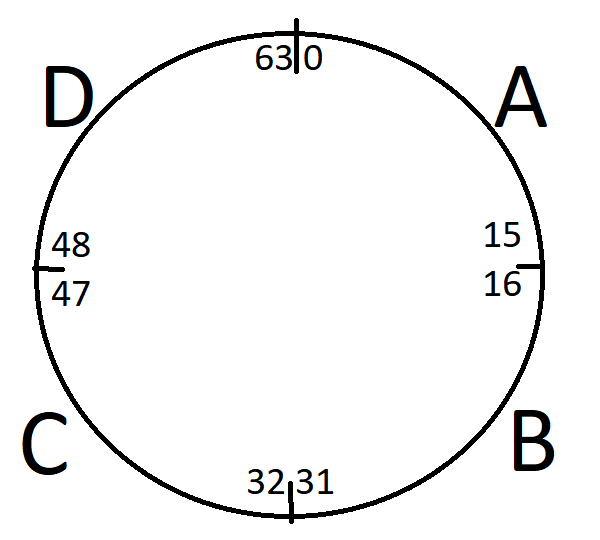
\includegraphics{fig/hashring.png}
    \caption{Eksempel på konsistent hashring i Project Voldemort. Node A lagrer nøkler med hashverdi 0--15, B lagrer nøkler hvis hashverdi er mellom 16 og 31, C lagrer nøkler hvis hashverdi er mellom 32 og 47, og D lagrer nøkler hvis hashverdi er mellom 48 og 63.}
    \label{fig4}
\end{figure}

Den logiske strukturen til likemannsnettverket av databasenoder i Voldemort har formen til en ring. Denne ringen består av en stor mengde diskrete posisjoner, verdiområdet til en hashfunksjon \emph{h}. Hver node som deltar i databaseklyngen tildeles en gruppe av disse punktene i ringen. \emph{h} brukes til å finne ringposisjonen til en nøkkel \emph{k}. Den noden hvis tilordnede mengde av hashverdier inneholder \emph{h(k)} blir den som lagrer det assosierte dataobjektet til \emph{k}.

Den konsistente hashalgoritmen og ringstrukturen til likemannsnettverket realiserer datareplikering ved å legge antallet påkrevde replikaer, per quorumkonfigurasjonen, på \underline{etterfølgende} noder i ringen, med sola \citep{elmasri2014}. Per \ref{fig4} og konfigurasjonen N=3 vil eksempelvis alle dataobjekter som hashes til node A også kopieres til node B og C.
\ldots



\cleardoublepage

% Hovedkjelder: sadalage2013; pensum fra egne fag

